\chapter{ZipPy: A Simple Python 3 for the JVM}
\label{chp:ch3-zippy}

Abstract syntax trees, ASTs, are the simplest and most natural ways to implement programming languages.
They do not require an additional translation step that linearizes ASTs produced by the parser to bytecode or other forms of internal representations.
They also lend themselves well to optimizations that are particularly beneficial to highly dynamic languages like Python.

We present ZipPy, a Python 3 implementation that is hosted on the JVM.
ZipPy incorporates recent works on self-optimizing AST interpreters for the JVM.
Our work however focuses on high level guest language features that are distinct in Python and
how well we can fit them onto the existing optimizing AST interpreter framework.

\section{Python on Truffle}

\begin{figure}[t]
\centering
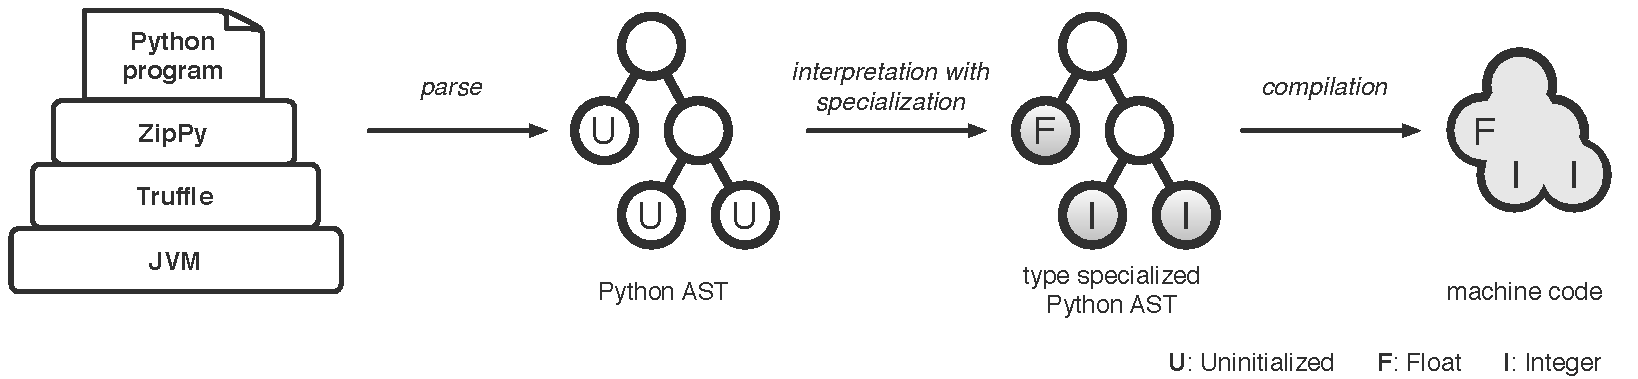
\includegraphics[scale=.6]{figures/ch3-python-on-truffle.pdf}
\caption{Python on Truffle}
\label{fig:python-on-truffle}
\end{figure}

In principle, ``everything'' can change at any moment in dynamic language programs.
This dynamic nature is the major impediment to ahead-of-time optimization.
In practice, however, programmers tend to minimize the rate of change, which makes the code highly predictable.
Types, for instance, typically remain stable between successive executions of a particular operation instance.
Deutsch and Schiffman report that speculative type specialization succeeds $95\%$ of the time in their classic Smalltalk-80 implementation~\cite{Deutsch1984}.

Truffle is a self-optimizing runtime system that makes it easy to perform type specialization for dynamic languages running on top of the JVM~\cite{Wurthinger+13}.
It allows language implementers to implement their guest language by writing an AST interpreter using Java.
An interpreter written in this way enjoys low cost type specialization via automatic node rewriting~\cite{Wurthinger+12,Brunthaler2010inca,Brunthaler2010quickening}.
AST node rewriting collects runtime type information, and speculatively replaces the existing nodes with specialized and more efficient ones.
Subsequently, Truffle just-in-time compiles the specialized AST, written in Java, directly to machine code using the underlying Java compiler.
Upon a type mis-speculation, the specialized AST node handles the type change by replacing itself with a more generic one.
The node replacement triggers deoptimization from the compiled code and transfers execution back to the interpreter.
If the re-specialized AST stays stable, Truffle can again compile it to machine code.

Our system, ZipPy, is a full-fledged prototype Python 3 implementation built atop Truffle.
It leverages Truffle's type specialization feature and its underlying compilation infrastructure (see Figure~\ref{fig:python-on-truffle}).
This architecture helps ZipPy outperform Python implementations that either do not exploit runtime type specialization or lack a just-in-time compiler.
However, Truffle has no knowledge about specific high level guest language semantics, like generators in Python.
Further performance exploration of a guest language will mainly benefit from better insights on distinct features of the language and
making better use of the host compiler based on those insights.
In this thesis we focus on guest language level optimizations we added to ZipPy.

ZipPy benefits from the Truffle framework in two ways.
First, Truffle's Java annotation based domain specific language (DSL) greatly simplifies the implementation of type specialization in dynamic languages like Python~\cite{Humer+2014}.
Second, Truffle bridges the gap between the hosted AST interpreter and the underlying Java JIT compiler.
It empowers the hosted interpreter with the performance of a custom compiler without having the hosted VM implementers to actually write a compiler.
The end performance one could achieve on Truffle usually surpasses that of a custom build class file compiler not to mention the upfront cost of building such compiler.

However, Truffle cannot automatically optimize guest languages.
It requires understandings of the Java compiler internals to make better use of the framework.
In this Chapter we describe the design choices we made to retrofit the core part of the Python language onto Truffle's execution model.

\section{Fast Arithmetics Via Type Specialization}
\label{sec:ch3-fast-arithmetics}

Arithmetic operations are fundamental constructs of a programming language.
It is challenging to implement efficient arithmetic operations in a dynamically typed langauge like Python.
In this Section, we explain how we utilize Truffle to enable fast arithmetics in ZipPy.

\subsection{Numeric Types}
\label{sec:numeric-types}

\begin{figure}[t]
\centering
\subfigure[Numeric types in Python 3] {
  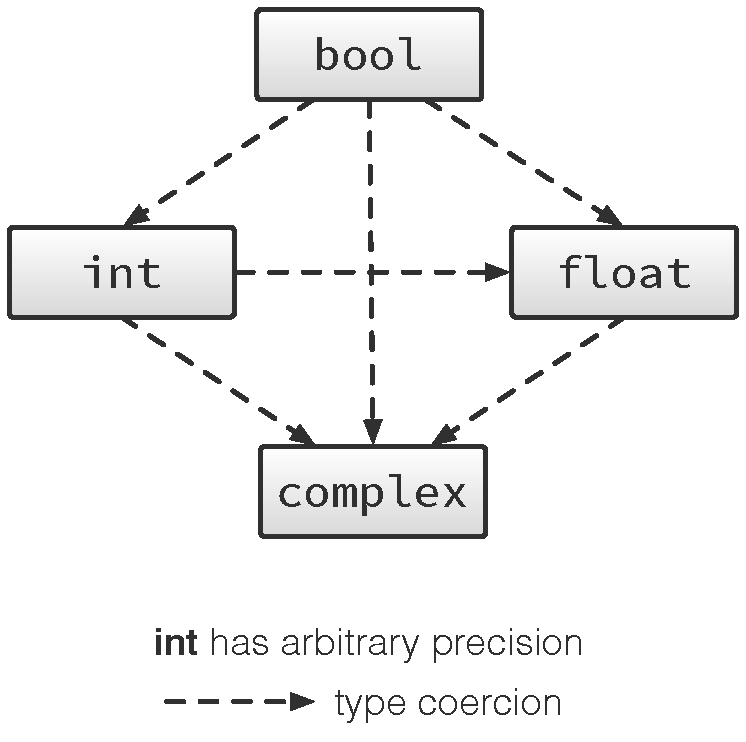
\includegraphics[scale=.4]{figures/ch3-numeric-types-python.pdf}
  \label{fig:numeric-types-python}
}
\subfigure[Boxed representation] {
  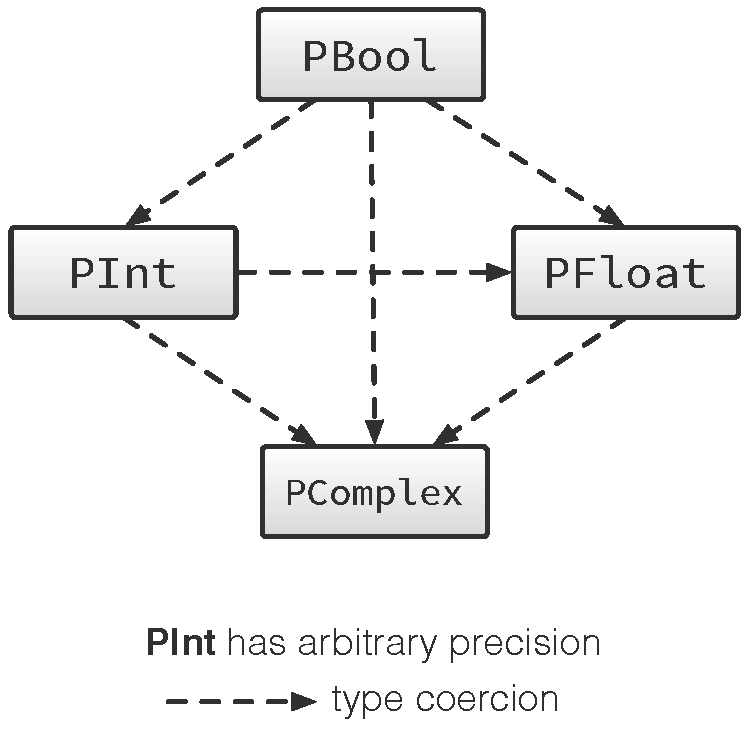
\includegraphics[scale=.4]{figures/ch3-numeric-types-boxed.pdf}
  \label{fig:numeric-types-boxed}
}
\subfigure[Unboxed representation] {
  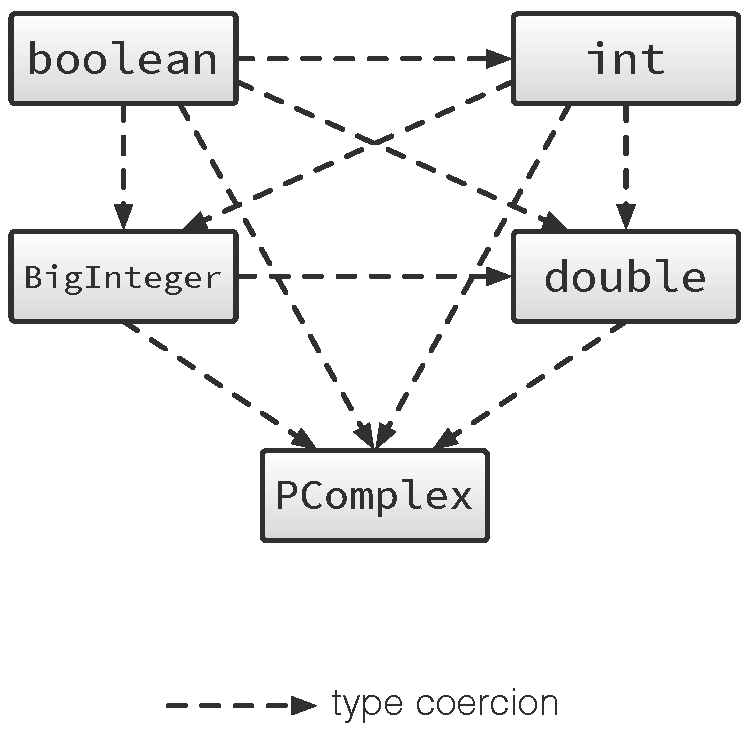
\includegraphics[scale=.4]{figures/ch3-numeric-types-unboxed.pdf}
  \label{fig:numeric-types-unboxed}
}
\caption{Numeric types in ZipPy}
\label{fig:numeric-types-zippy}
\end{figure}

Numeric types are the most commonly used built-in types in Python.
It is essential to have efficient data representation for the built-in numeric types in Python.
Figure~\ref{fig:numeric-types-python} illustrates the four numeric types in Python: booleans, integers, floating point numbers and complex numbers.
The figure also depicts type coercion rules between those types.
Note that the value range of an integer in Python 3 is unbounded.

All data in Python is an object.
So are all the numbers.
A straight-forward way to model the built-in numeric types, which is similar to the one in CPython, is to implement them as boxed Java objects.
As shown in Figure~\ref{fig:numeric-types-boxed}, in the boxed representation ZipPy uses a Java object to represent a Python number.
The object boxes the actual value of the number as a field.
To preserve the unbounded integer semantics, a \texttt{PInt} uses a \texttt{BigInteger} field to store its integer value (Figure~\ref{fig:numeric-types-boxed}).
For all the arithmetic operation nodes in ZipPy, we specify the type specializations in the order that ensures the correct type coercion rules.

ZipPy uses another unboxed data representation for numbers to achieve fast arithmetic operation.
Essentially we map Python numeric types to Java primitive types as long as possible.
For instance, initially ZipPy uses a Java \texttt{int} to represent a Python \texttt{int}.
For all arithmetic operations that consume unboxed numbers, as long as the result does not overflow, ZipPy keep their result remain unboxed.
Object operations such as attribute access trigger lazy boxing that coverts a number from the unboxed representation to the boxed one.
To handle the unbound integer semantics, ZipPy use \texttt{BigInteger} to model integers with bigger values in addition to Java primitive \texttt{int}.

\subsection{Applying Type Specializations}

\begin{figure}[t]
\centering
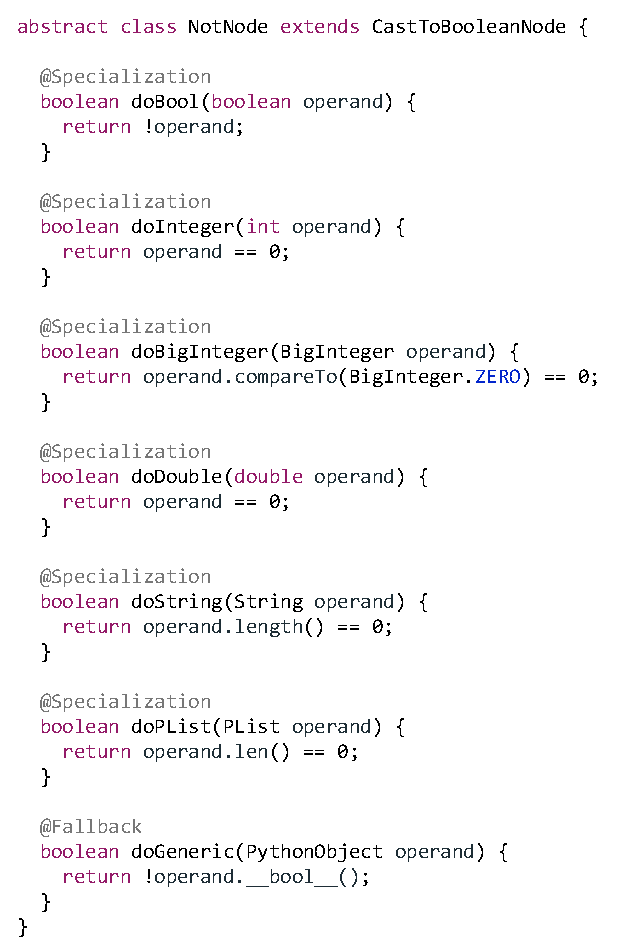
\includegraphics[scale=.9]{figures/ch3-not-node-code.pdf}
\caption{Implementation of \texttt{NotNode} in ZipPy}
\label{fig:not-node-code}
\end{figure}

\begin{figure}[t]
\centering
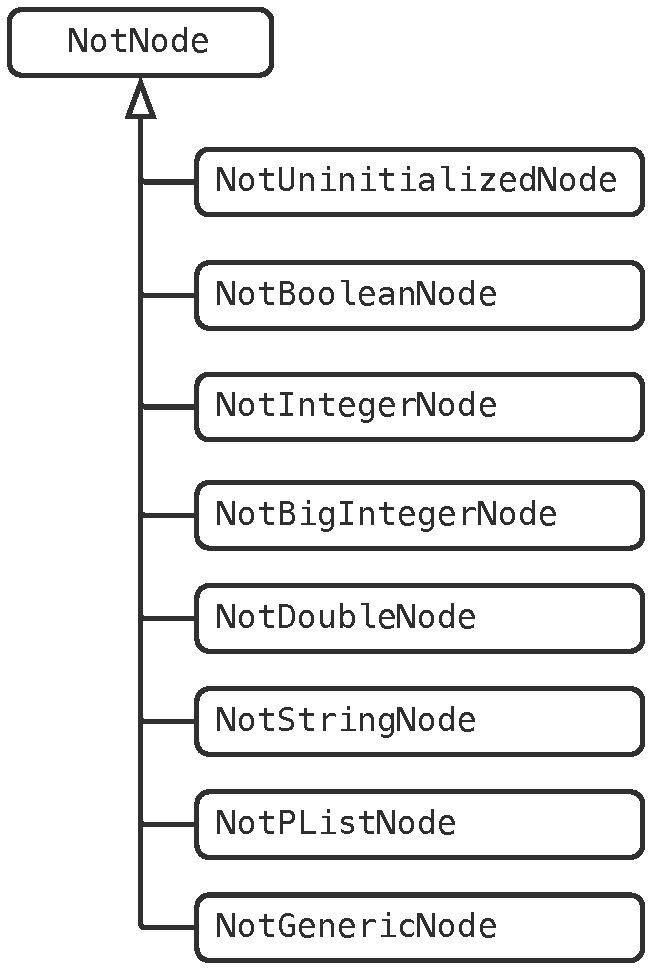
\includegraphics[scale=.5]{figures/ch3-not-node-derivatives.pdf}
\caption{Derivatives of \texttt{NotNode} in ZipPy}
\label{fig:not-node-derivatives}
\end{figure}

Truffle provides a Java annotation based source code generation engine.
Hosted VM implementers can use this engine to automatically generate type specialized derivatives for their AST interpreters.
Derivative generation is an essential but tedious part of applying type specializations.
This code generation process requires minimum boilerplate code from the hosted VM implementers and helps them to focus on the core logic of their interpreter.

\texttt{not} is a unary arithmetic operation in Python.
The operation evaluates the given expression to a boolean value and returns the inversion of that value.
Similar to other arithmetic operations, ZipPy implements \texttt{not} as a single AST node.
Figure~\ref{fig:not-node-code} illustrates the implementation of the \texttt{NotNode} in ZipPy using Truffle's DSL (simplified for brevity).
Note that each method annotated using \texttt{@Specialization} represents a type specialized derivative of the \texttt{NotNode}.
For instance, the method \texttt{doInteger} and \texttt{doDouble} implement the \texttt{not} operation for integers and floating point numbers.
We will explain in~\ref{sec:numeric-types} about the reason why we specialize against Java primitive types instead of boxed representations of numeric types in Python.
\texttt{@Fallback} denotes the generic version of the \texttt{not} operand.

Truffle's code generation engine produces the actual implementation of the derivative nodes.
Figure~\ref{fig:not-node-derivatives} shows the derivative classes produced by Truffle.
It generates a class for each method annotated with \texttt{@Specialization} in Figure~\ref{fig:not-node-code}.
The derivative nodes perform node rewriting based type specialization at runtime.
As shown in Figure~\ref{fig:python-on-truffle}, a \texttt{NotNode} starts with the uninitialized version.
At runtime, the node rewrites itself to a derivative that matches the type of the incoming operand.
The rewrite follows the order of the classes shown in Figure~\ref{fig:not-node-derivatives} from the top to the bottom.
If no matching derivative is found, the node rewrites to \texttt{NodeGenericNode}, which perform the generic routine for the \texttt{not} operation.

\section{Efficient Data Representation for Composite Data Types}

Python provides a rich set of built-in composite data types including \texttt{list}s, \texttt{tuple}s, \texttt{set}s, and \texttt{dict}s.
Jython uses a straight-forward approach that uses the existing collection types in the Java development kit (JDK) to implement these data types.
This approach is simple to implement but adds runtime cost to the use of the data types.
When adding an element to a Java generics based collection type, the JVM performs auto-boxing on the primitive types to their corresponding object wrapper classes.
Auto-boxing ensures that every element in a collection type is of reference type.
This design simplifies garbage collection in Java, since the garbage collector does not have to distinguish between reference type and value type for members of collection types.
However, auto-boxing involves heap allocation and additional memory accesses, and it slows down accesses to composite data types in Jython.

\subsection{Unboxed Sequence Storage}

\begin{figure}[ht]
\centering
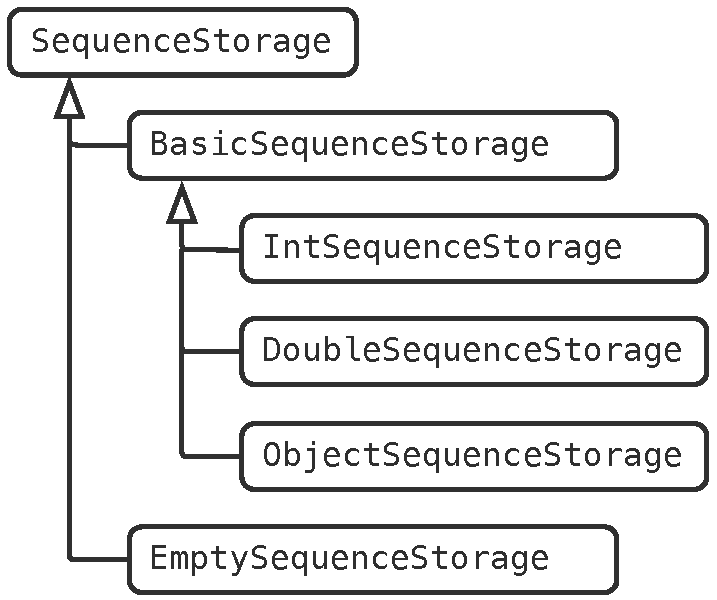
\includegraphics[scale=.5]{figures/ch3-sequence-storage-types.pdf}
\caption{Sequence storage types in ZipPy}
\label{fig:sequence-storage-types}
\end{figure}

ZipPy employs more efficient data representations for Python composite or sequence data types to avoid auto-boxing.
Unlike \texttt{tuple}s, programmers tend to use \texttt{list}s in a homogeneous way meaning that elements of a \texttt{list} are usually of the same type.
Therefore, we can speculatively stores a list of integers, for instance, in a Java primitive \texttt{int} array to avoid auto-boxing.
In ZipPy, a \texttt{list} stores its elements in a \texttt{SequenceStorage} object that dynamically switches between different concrete data representations.
Figure~\ref{fig:sequence-storage-types} shows the different \texttt{SequenceStorage} types used in ZipPy.
For instance, a list of Python integers uses a \texttt{IntSequenceStorage} to store the integers in a Java primitive \texttt{int} array assuming that the element types will stay the same.
As long as the assumption holds, ZipPy specializes accesses of the integer list and avoids auto-boxing altogether.
Once the assumption becomes invalid, the list automatically converts its \texttt{SequenceStorage} to the next matching type to preserve semantics.

\subsection{Profiling-based List Literal Specialization}

\begin{figure}[ht]
\centering
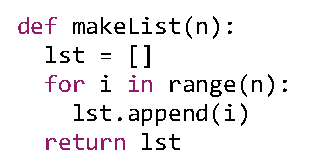
\includegraphics[scale=.9]{figures/ch3-list-construction-loop-code.pdf}
\caption{List construction loop}
\label{fig:list-construction-loop-code}
\end{figure}

\begin{figure}[t]
\centering
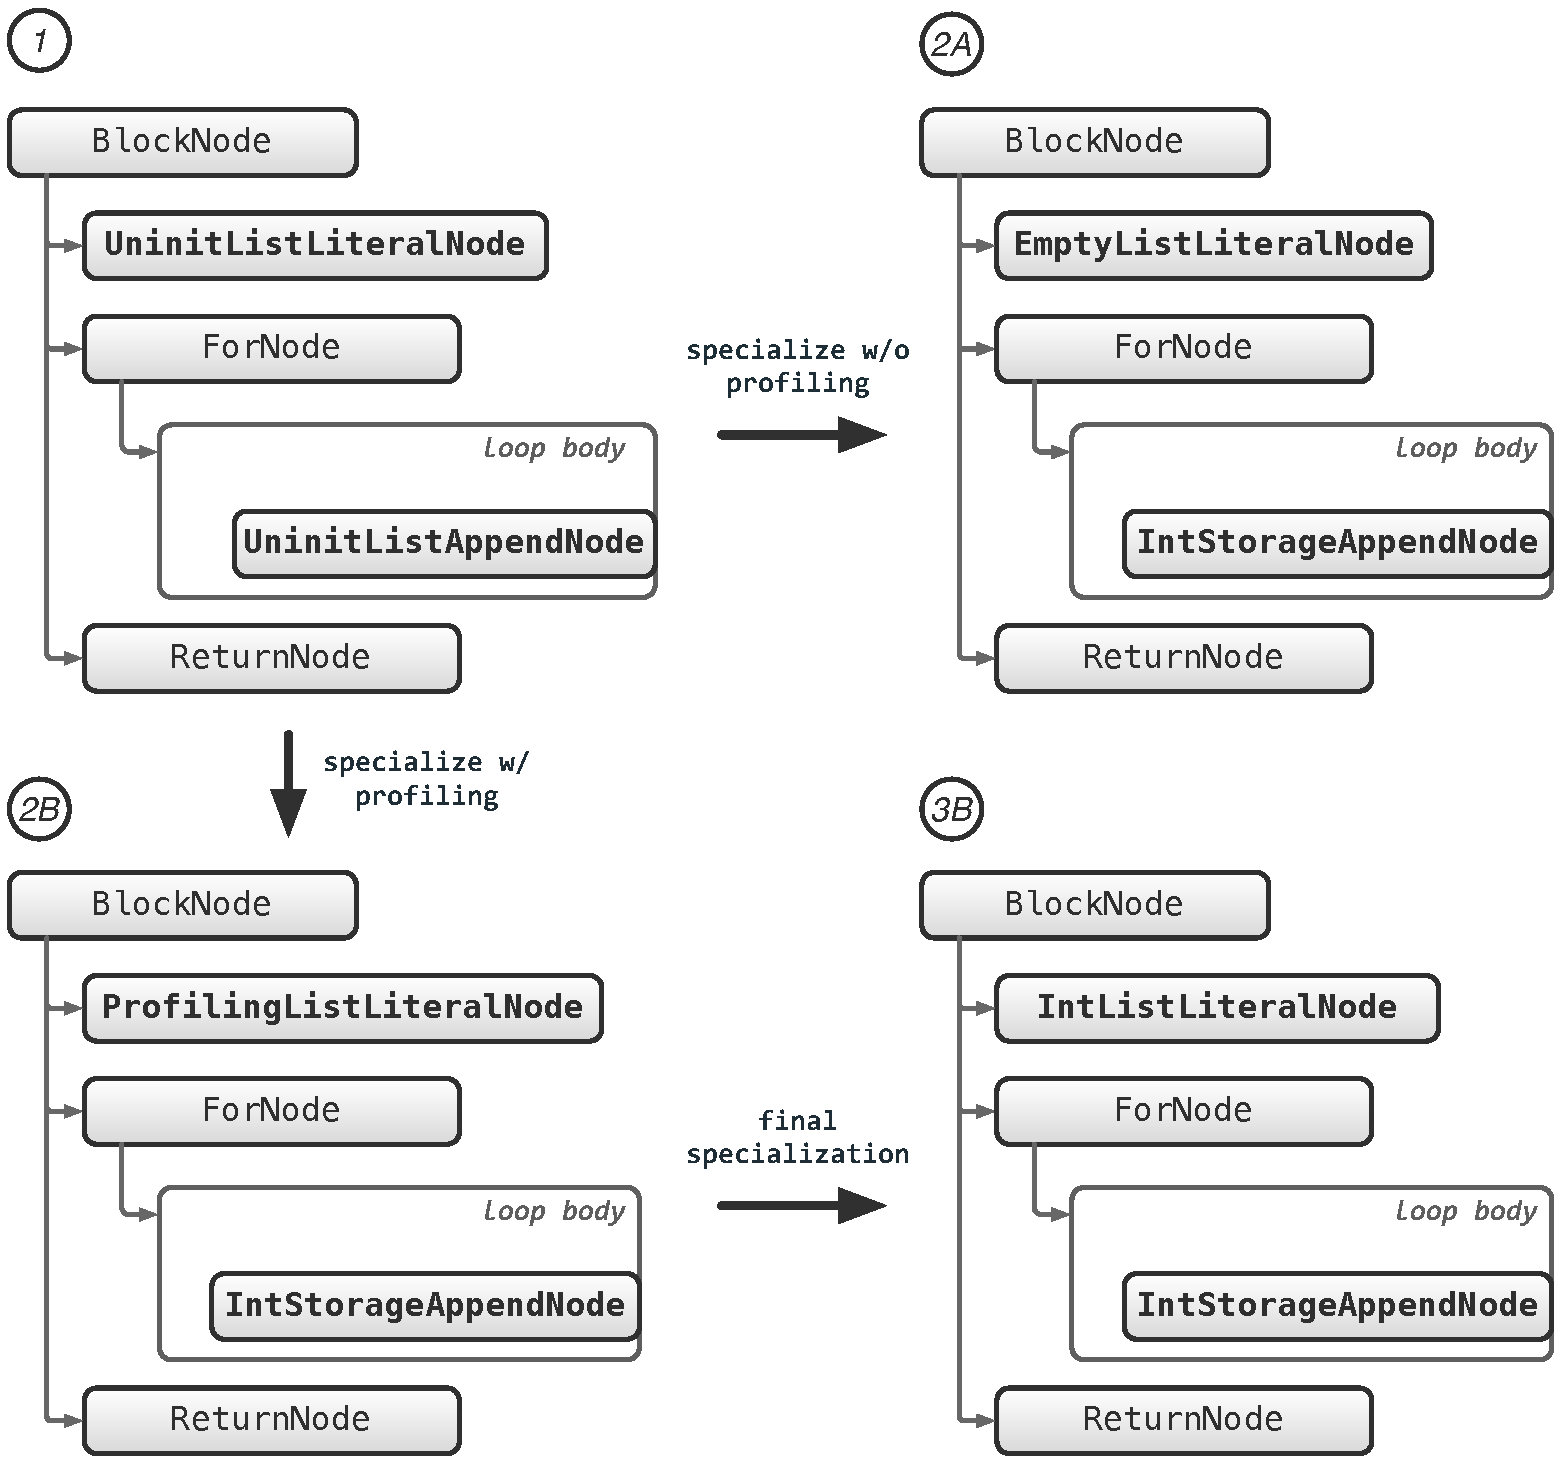
\includegraphics[scale=.55]{figures/ch3-empty-list-storage-profiling.pdf}
\caption{List literal specialization}
\label{fig:empty-list-storage-profiling}
\end{figure}

ZipPy enables the use of unboxed sequence storages by specializing Python list constructions.
More specifically we create type specialized derivatives for list constructor calls and list literals.
When a list literal creates a list that can use a more efficient sequence storage type, we specialize it to a typed list literal
that always try to create a list using an unboxed sequence storage type.

However, some times the list construction site does not have enough information about the elements going into the list at a later point.
For instance, what we often see in Python programs is a pattern similar to the code snippet shown in Figure~\ref{fig:list-construction-loop-code}.
The shown program first instantiates an empty list and then populates the list one element at a time using a loop.
The for range loop in Figure~\ref{fig:list-construction-loop-code} appends integers to list \texttt{lst},
which ideally should use an \texttt{IntSequenceStorage} to store its elements to avoid auto-boxing.

Figure~\ref{fig:empty-list-storage-profiling} illustrates the simplified ASTs of the \texttt{makeList} function shown in Figure~\ref{fig:list-construction-loop-code}.
The AST labeled as \textsf{1} is the initial version with both the \texttt{ListLiteralNode} and \texttt{ListAppendNode} uninitialized.
If we simply specialize the \texttt{ListLiteralNode} base on type information available locally, we will replace it with an \texttt{EmptyListLiteralNode} (\textsf{2A} in Figure~\ref{fig:empty-list-storage-profiling}).
The \texttt{EmptyListLiteralNode} returns a list backed by an \texttt{EmptySequenceStorage}.
Subsequently the \texttt{ListAppendNode} in the loop body specializes itself to an \texttt{IntStorageAppendNode} and switches the list's storage to an \texttt{IntSequenceStorage}.
The remaining iterations of the loop does not introduce changes to the AST and populates and populates the list using an efficient data representation.
However, if \texttt{makeList} is invoked again, the above mentioned specializations will alter.
Note that the \texttt{EmptyListLiteralNode} always return a list using \texttt{EmptySequenceStorage}.
This storage type is not expected by the \texttt{IntStorageAppendNode} in the loop body and will trigger a re-specialization that generalizes the list storage type to an boxed one.
The reason of this action is that the previous specialization to \texttt{IntSequenceStorage} become unstable.
Therefore, the node need to give up the current specialization, and rewrites itself to the next matching derivative version.
In short, the straight forward specialization can not properly handle empty list instantiation.

Alternatively, we could add an intermediate step when specializing list literals.
As shown in Figure~\ref{fig:empty-list-storage-profiling}, ZipPy first specializes the \texttt{UninitializedListLiteralNode} in \textsf{1} to the \texttt{Profili\-ngListLiteralNode} in \textsf{2B}.
The \texttt{ProfilingListLiteralNode} keeps a reference to the list it previously instantiated.
Upon the second execution of function \texttt{makeList}, the \texttt{ProfilingLis\-tLiteralNode} rewrites itself by looking at the storage type of the previously created list.
It performs the final specialization to the derivative version that matches the previous list assuming that the next list is most likely to have the same storage type.
This step results in the stable AST \textsf{3B} shown in Figure~\ref{fig:empty-list-storage-profiling}.
By using profiling based non-local type feedback, ZipPy is able to optimize list accesses for more complicated list construction pattern in Python programs.


\section{Control Flow Specializations}

\subsection{For Loop Specializations}

\begin{figure}
\centering
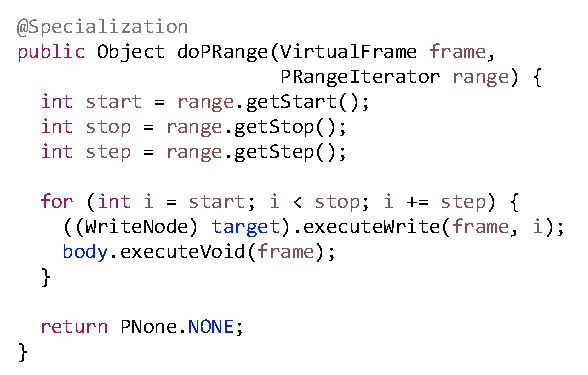
\includegraphics[scale=.9]{figures/ch3-for-range-node-code.pdf}
\caption{For loop specialization for range iterators}
\label{fig:for-range-node}
\end{figure}

Unlike the way other languages use it, for statements in Python iterate over a sequence of items, like a list or a string, in the order that they appear in the sequence.
ZipPy models Python control flow using Java control flow constructs.
Naturally it uses Java loops to construct for loops in Python.
If we abstract a for loop in Python as an operation, the only input operand of this operation is the sequence flowing into the loop.
Evidently we could apply type specializations on for loops like we did to the other operations in ZipPy.

Figure~\ref{fig:for-range-node} shows a specialization we added to the \texttt{ForNode} for \texttt{PRangeIterators} in ZipPy.
In Python the built-in \texttt{range} function generates an iterable containing arithmetic progressions that can be used to iterate over a sequence of numbers.
A for loop over a range iterator, or a for range loop like the one shown in Figure~\ref{fig:list-construction-loop-code}, is the most common use of for loops among Python programs.
The \texttt{doPRange} method shown in Figure~\ref{fig:for-range-node} completely unboxes the incoming \texttt{PRangeIterator} into a few primitive integer indices.
This approach effectively lower the semantics level of a for range loop in Python to a straight forward for loop in Java.
The for range specialization not only minimizes the loop overhead on the JVM, it also enables more advanced loop optimizations like loop unrolling for the Java compiler.

\subsection{List Comprehensions}

\begin{figure}[h]
\centering
\subfigure[original] {
  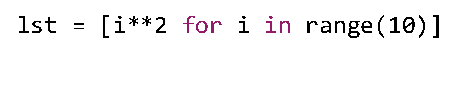
\includegraphics[scale=.9]{figures/ch3-list-comp-code.pdf}
  \label{fig:list-comp-code}
}
\subfigure[desugared] {
  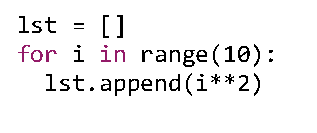
\includegraphics[scale=.9]{figures/ch3-list-comp-desugared-code.pdf}
  \label{fig:list-comp-desugared-code}
}
\caption{List comprehensions}
\label{fig:list-comp}
\end{figure}

List comprehension provides a concise way to construct lists in Python.
It allows expressing the construction of a list from another sequence in one compact expression.
Figure~\ref{fig:list-comp-code} illustrates the use of list comprehension to create the list \texttt{lst} that consists of the square of $0$ to $9$.
Figure~\ref{fig:list-comp-desugared-code} shows the desugared equivalence of the shown list comprehension.
Note that we can always expand a list comprehension to an explicit loop that creates the same list in Python.
When parsing a list comprehension, ZipPy applies a similar desugaring process as shown in Figure~\ref{fig:list-comp}.
It automatically expands the list comprehension to an AST that is equivalent to what is shown in Figure~\ref{fig:list-comp-desugared-code}.
This transformation enables further optimizations described previously in this section such as unboxed data representation for the created list, proper type specialization and compiler optimizations of the expanded loop.
In summary, list comprehension desugaring eliminates the performance overhead introduced by the concise syntax of list comprehension, and enables efficient list creations in ZipPy.

\section{Discussion}
ZipPy is the first full-fledged Python 3 protype running atop the Java virtual machine.
Our implementation applies type specialization using Truffle by replacing generic AST nodes with type-specialized ones during execution.
We also present efficient supports of composite data types and loops that specifically benefit Python programs.
The techniques we discussed in this Chapter provide a performant basis that includes the imperative subset of the Python language.
